
\documentclass[letterpaper,hide notes,xcolor={table,svgnames},pdftex,10pt]{beamer}
\def\showexamples{t}

\usecolortheme{crane}
\setbeamertemplate{navigation symbols}{}

\usetheme{MyPittsburgh}
\usepackage{hyperref}
\usepackage{graphicx,xspace}
\usepackage[normalem]{ulem}
\usepackage{multicol}
\usepackage{amsmath,amssymb,amsthm,graphicx,xspace}
\newcommand\SF[1]{$\bigstar$\footnote{SF: #1}}

\usepackage[sfdefault,lf]{carlito}
\usepackage[T1]{fontenc}
\usepackage[scaled]{beramono}
\usepackage{tikzpagenodes}
\newcommand{\Rplus}{\protect\hspace{-.1em}\protect\raisebox{.35ex}{\small{\small\textbf{+}}}}
\newcommand{\Cpp}{\mbox{C\Rplus\Rplus}\xspace}

\newcounter{tmpnumSlide}
\newcounter{tmpnumNote}

\newcommand\mnote[1]{%
	\addtocounter{tmpnumSlide}{1}
	\ifdefined\showcues {~\tiny\fbox{\arabic{tmpnumSlide}}}\fi
	\note{\setlength{\parskip}{1ex}\addtocounter{tmpnumNote}{1}\textbf{\Large \arabic{tmpnumNote}:} {#1\par}}}

\newcommand\mmnote[1]{\note{\setlength{\parskip}{1ex}#1\par}}


\newcommand\mquestion[2]{{~\color{red}\fbox{?}}\note{\setlength{\parskip}{1ex}\par{\Large \textbf{?}} #1} \note{\setlength{\parskip}{1ex}\par{\Large \textbf{A}} #2\par}\ifdefined \presentationonly \pause \fi}

\newcommand\blackboard[1]{%
	\ifdefined   \showblackboard
		{#1}
	\else {\begin{center} \fbox{\colorbox{blue!30}{%
						\begin{minipage}{.95\linewidth}%
							\hspace{\stretch{1}} Some space intentionally left blank; done at the blackboard.%
						\end{minipage}}}\end{center}}%
	\fi%
}

\usepackage{listings}
\lstset{%
	keywordstyle=\bfseries,
	aboveskip=15pt,
	belowskip=15pt,
	captionpos=b,
	identifierstyle=\ttfamily,
	frame=lines,
	numbers=left, basicstyle=\scriptsize, numberstyle=\tiny, stepnumber=0, numbersep=2pt}

\usepackage{siunitx}
\newcommand\sius[1]{\num[group-separator = {,}]{#1}\si{\micro\second}}
\newcommand\sims[1]{\num[group-separator = {,}]{#1}\si{\milli\second}}
\newcommand\sins[1]{\num[group-separator = {,}]{#1}\si{\nano\second}}
\sisetup{group-separator = {,}, group-digits = true}

%% -------------------- tikz --------------------
\usepackage{tikz}
\usetikzlibrary{positioning}
\usetikzlibrary{arrows,backgrounds,automata,decorations.shapes,decorations.pathmorphing,decorations.markings,decorations.text}

\tikzstyle{place}=[circle,draw=blue!50,fill=blue!20,thick, inner sep=0pt,minimum size=6mm]
\tikzstyle{transition}=[rectangle,draw=black!50,fill=black!20,thick, inner sep=0pt,minimum size=4mm]

\tikzstyle{block}=[rectangle,draw=black, thick, inner sep=5pt]
\tikzstyle{bullet}=[circle,draw=black, fill=black, thin, inner sep=2pt]

\tikzstyle{pre}=[<-,shorten <=1pt,>=stealth',semithick]
\tikzstyle{post}=[->,shorten >=1pt,>=stealth',semithick]
\tikzstyle{bi}=[<->,shorten >=1pt,shorten <=1pt, >=stealth',semithick]

\tikzstyle{mut}=[-,>=stealth',semithick]

\tikzstyle{treereset}=[dashed,->, shorten >=1pt,>=stealth',thin]

\usepackage{ifmtarg}
\usepackage{xifthen}
\makeatletter
% new counter to now which frame it is within the sequence
\newcounter{multiframecounter}
% initialize buffer for previously used frame title
\gdef\lastframetitle{\textit{undefined}}
% new environment for a multi-frame
\newenvironment{multiframe}[1][]{%
	\ifthenelse{\isempty{#1}}{%
		% if no frame title was set via optional parameter,
		% only increase sequence counter by 1
		\addtocounter{multiframecounter}{1}%
	}{%
		% new frame title has been provided, thus
		% reset sequence counter to 1 and buffer frame title for later use
		\setcounter{multiframecounter}{1}%
		\gdef\lastframetitle{#1}%
	}%
	% start conventional frame environment and
	% automatically set frame title followed by sequence counter
	\begin{frame}%
		\frametitle{\lastframetitle~{\normalfont(\arabic{multiframecounter})}}%
		}{%
	\end{frame}%
}
\makeatother

\makeatletter
\newdimen\tu@tmpa%
\newdimen\ydiffl%
\newdimen\xdiffl%
\newcommand\ydiff[2]{%
	\coordinate (tmpnamea) at (#1);%
	\coordinate (tmpnameb) at (#2);%
	\pgfextracty{\tu@tmpa}{\pgfpointanchor{tmpnamea}{center}}%
	\pgfextracty{\ydiffl}{\pgfpointanchor{tmpnameb}{center}}%
	\advance\ydiffl by -\tu@tmpa%
}
\newcommand\xdiff[2]{%
	\coordinate (tmpnamea) at (#1);%
	\coordinate (tmpnameb) at (#2);%
	\pgfextractx{\tu@tmpa}{\pgfpointanchor{tmpnamea}{center}}%
	\pgfextractx{\xdiffl}{\pgfpointanchor{tmpnameb}{center}}%
	\advance\xdiffl by -\tu@tmpa%
}
\makeatother
\newcommand{\copyrightbox}[3][r]{%
	\begin{tikzpicture}%
		\node[inner sep=0pt,minimum size=2em](ciimage){#2};
		\usefont{OT1}{phv}{n}{n}\fontsize{4}{4}\selectfont
		\ydiff{ciimage.south}{ciimage.north}
		\xdiff{ciimage.west}{ciimage.east}
		\ifthenelse{\equal{#1}{r}}{%
			\node[inner sep=0pt,right=1ex of ciimage.south east,anchor=north west,rotate=90]%
			{\raggedleft\color{black!50}\parbox{\the\ydiffl}{\raggedright{}#3}};%
		}{%
			\ifthenelse{\equal{#1}{l}}{%
				\node[inner sep=0pt,right=1ex of ciimage.south west,anchor=south west,rotate=90]%
				{\raggedleft\color{black!50}\parbox{\the\ydiffl}{\raggedright{}#3}};%
			}{%
				\node[inner sep=0pt,below=1ex of ciimage.south west,anchor=north west]%
				{\raggedleft\color{black!50}\parbox{\the\xdiffl}{\raggedright{}#3}};%
			}
		}
	\end{tikzpicture}
}


%% --------------------

%\usepackage[excludeor]{everyhook}
%\PushPreHook{par}{\setbox0=\lastbox\llap{MUH}}\box0}

%\vspace*{\stretch{1}

%\setbox0=\lastbox \llap{\textbullet\enskip}\box0}

\setlength{\parskip}{\fill}

\newcommand\noskips{\setlength{\parskip}{1ex}}
\newcommand\doskips{\setlength{\parskip}{\fill}}

\newcommand\xx{\par\vspace*{\stretch{1}}\par}
\newcommand\xxs{\par\vspace*{2ex}\par}
\newcommand\tuple[1]{\langle #1 \rangle}
\newcommand\code[1]{{\sf \footnotesize #1}}
\newcommand\ex[1]{\uline{Example:} \ifdefined \presentationonly \pause \fi
	\ifdefined\showexamples#1\xspace\else{\uline{\hspace*{2cm}}}\fi}

\newcommand\ceil[1]{\lceil #1 \rceil}


\AtBeginSection[]
{
	\begin{frame}
		\frametitle{Outline}
		\tableofcontents[currentsection]
	\end{frame}
}



\pgfdeclarelayer{edgelayer}
\pgfdeclarelayer{nodelayer}
\pgfsetlayers{edgelayer,nodelayer,main}

\tikzstyle{none}=[inner sep=0pt]
\tikzstyle{rn}=[circle,fill=Red,draw=Black,line width=0.8 pt]
\tikzstyle{gn}=[circle,fill=Lime,draw=Black,line width=0.8 pt]
\tikzstyle{yn}=[circle,fill=Yellow,draw=Black,line width=0.8 pt]
\tikzstyle{empty}=[circle,fill=White,draw=Black]
\tikzstyle{bw} = [rectangle, draw, fill=blue!20,
text width=4em, text centered, rounded corners, minimum height=2em]

\newcommand{\CcNote}[1]{% longname
	This work is licensed under the \textit{Creative Commons #1 3.0 License}.%
}
\newcommand{\CcImageBy}[1]{%
	\includegraphics[scale=#1]{creative_commons/cc_by_30.pdf}%
}
\newcommand{\CcImageSa}[1]{%
	\includegraphics[scale=#1]{creative_commons/cc_sa_30.pdf}%
}
\newcommand{\CcImageNc}[1]{%
	\includegraphics[scale=#1]{creative_commons/cc_nc_30.pdf}%
}
\newcommand{\CcGroupBySa}[2]{% zoom, gap
	\CcImageBy{#1}\hspace*{#2}\CcImageNc{#1}\hspace*{#2}\CcImageSa{#1}%
}
\newcommand{\CcLongnameByNcSa}{Attribution-NonCommercial-ShareAlike}

\newenvironment{changemargin}[1]{% 
	\begin{list}{}{% 
		\setlength{\topsep}{0pt}% 
		\setlength{\leftmargin}{#1}% 
		\setlength{\rightmargin}{1em}
		\setlength{\listparindent}{\parindent}% 
		\setlength{\itemindent}{\parindent}% 
		      \setlength{\parsep}{\parskip}% 
		      }% 
		\item[]}{\end{list}}




\title{Lecture 22 --- Of Asgard and Hel }

\author{Jeff Zarnett \\ \small \texttt{jzarnett@uwaterloo.ca}}
\institute{Department of Electrical and Computer Engineering \\
	University of Waterloo}
\date{\today}


\begin{document}

\begin{frame}
	\titlepage

\end{frame}


\begin{frame}
	\frametitle{Yggdrasil, the World Tree}

	\begin{center}
		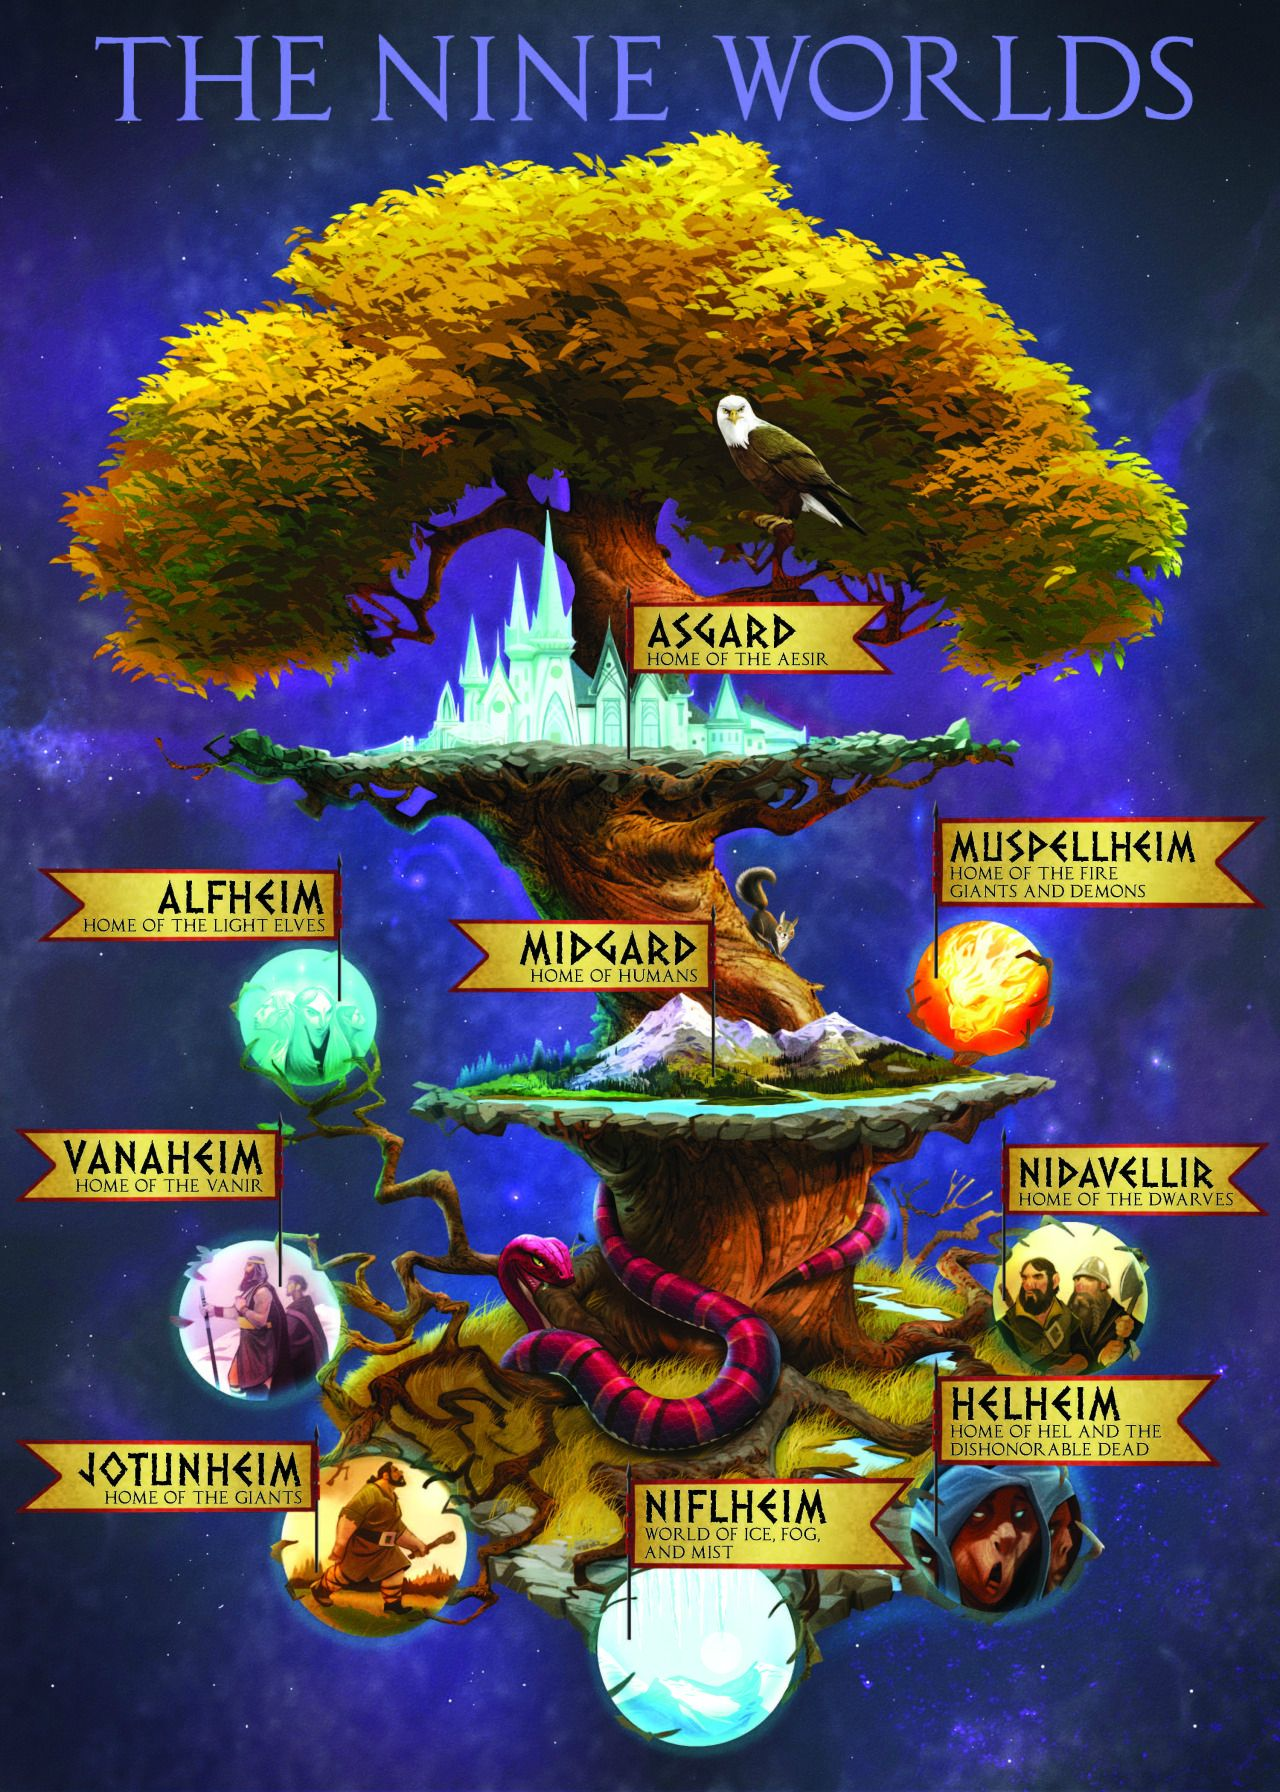
\includegraphics[width=0.5\textwidth]{images/Yggdrasil.jpg}
	\end{center}
	\hfill Image Credit: Rick Riordan, Magnus Chase and the Gods of Asgard
\end{frame}


\begin{frame}
	\frametitle{Ginnungagap}

	Everything came into creation in the gap between fire and ice, and the World Tree (Yggdrasil) connects the nine worlds.

	Asgard is the home of the \AE sir, the Norse gods.

	Helheim, or simply Hel, is the underworld where the dead go upon their death.

	In Hel or Asgard (it's not clear), there is Valhalla, hall of the honoured dead.

\end{frame}

\begin{frame}
	\frametitle{Carry We, Who Die In Battle...}

	Those who die in battle and are judged worthy will be carried to Valhalla by the Valkyries.

	There they will reside until they are called upon to aid in Odin's fight with the wolf Fenrir in Ragnar\"ok.

	humans live in the ``middle realm'', Midg\aa rd, surrounded by the serpent Jormungand, who will fight against Thor in  Ragnar\"ok.

	Thor will kill the serpent, but the serpent's poison will also finish off Thor.

\end{frame}

\begin{frame}
	\frametitle{Across the Rainbow Bridge, To Valhalla...}

	We're going to examine some very useful tools for programming called Valgrind and Helgrind (also Cachegrind).

	Where do they take their names from? Valgrind is the gateway to Valhalla; a gate that only the worthy can pass.

	Helgrind is the gateway to, well, Hel.
\end{frame}


\begin{frame}
	\frametitle{I may be interested in this subject...}

	\begin{center}
		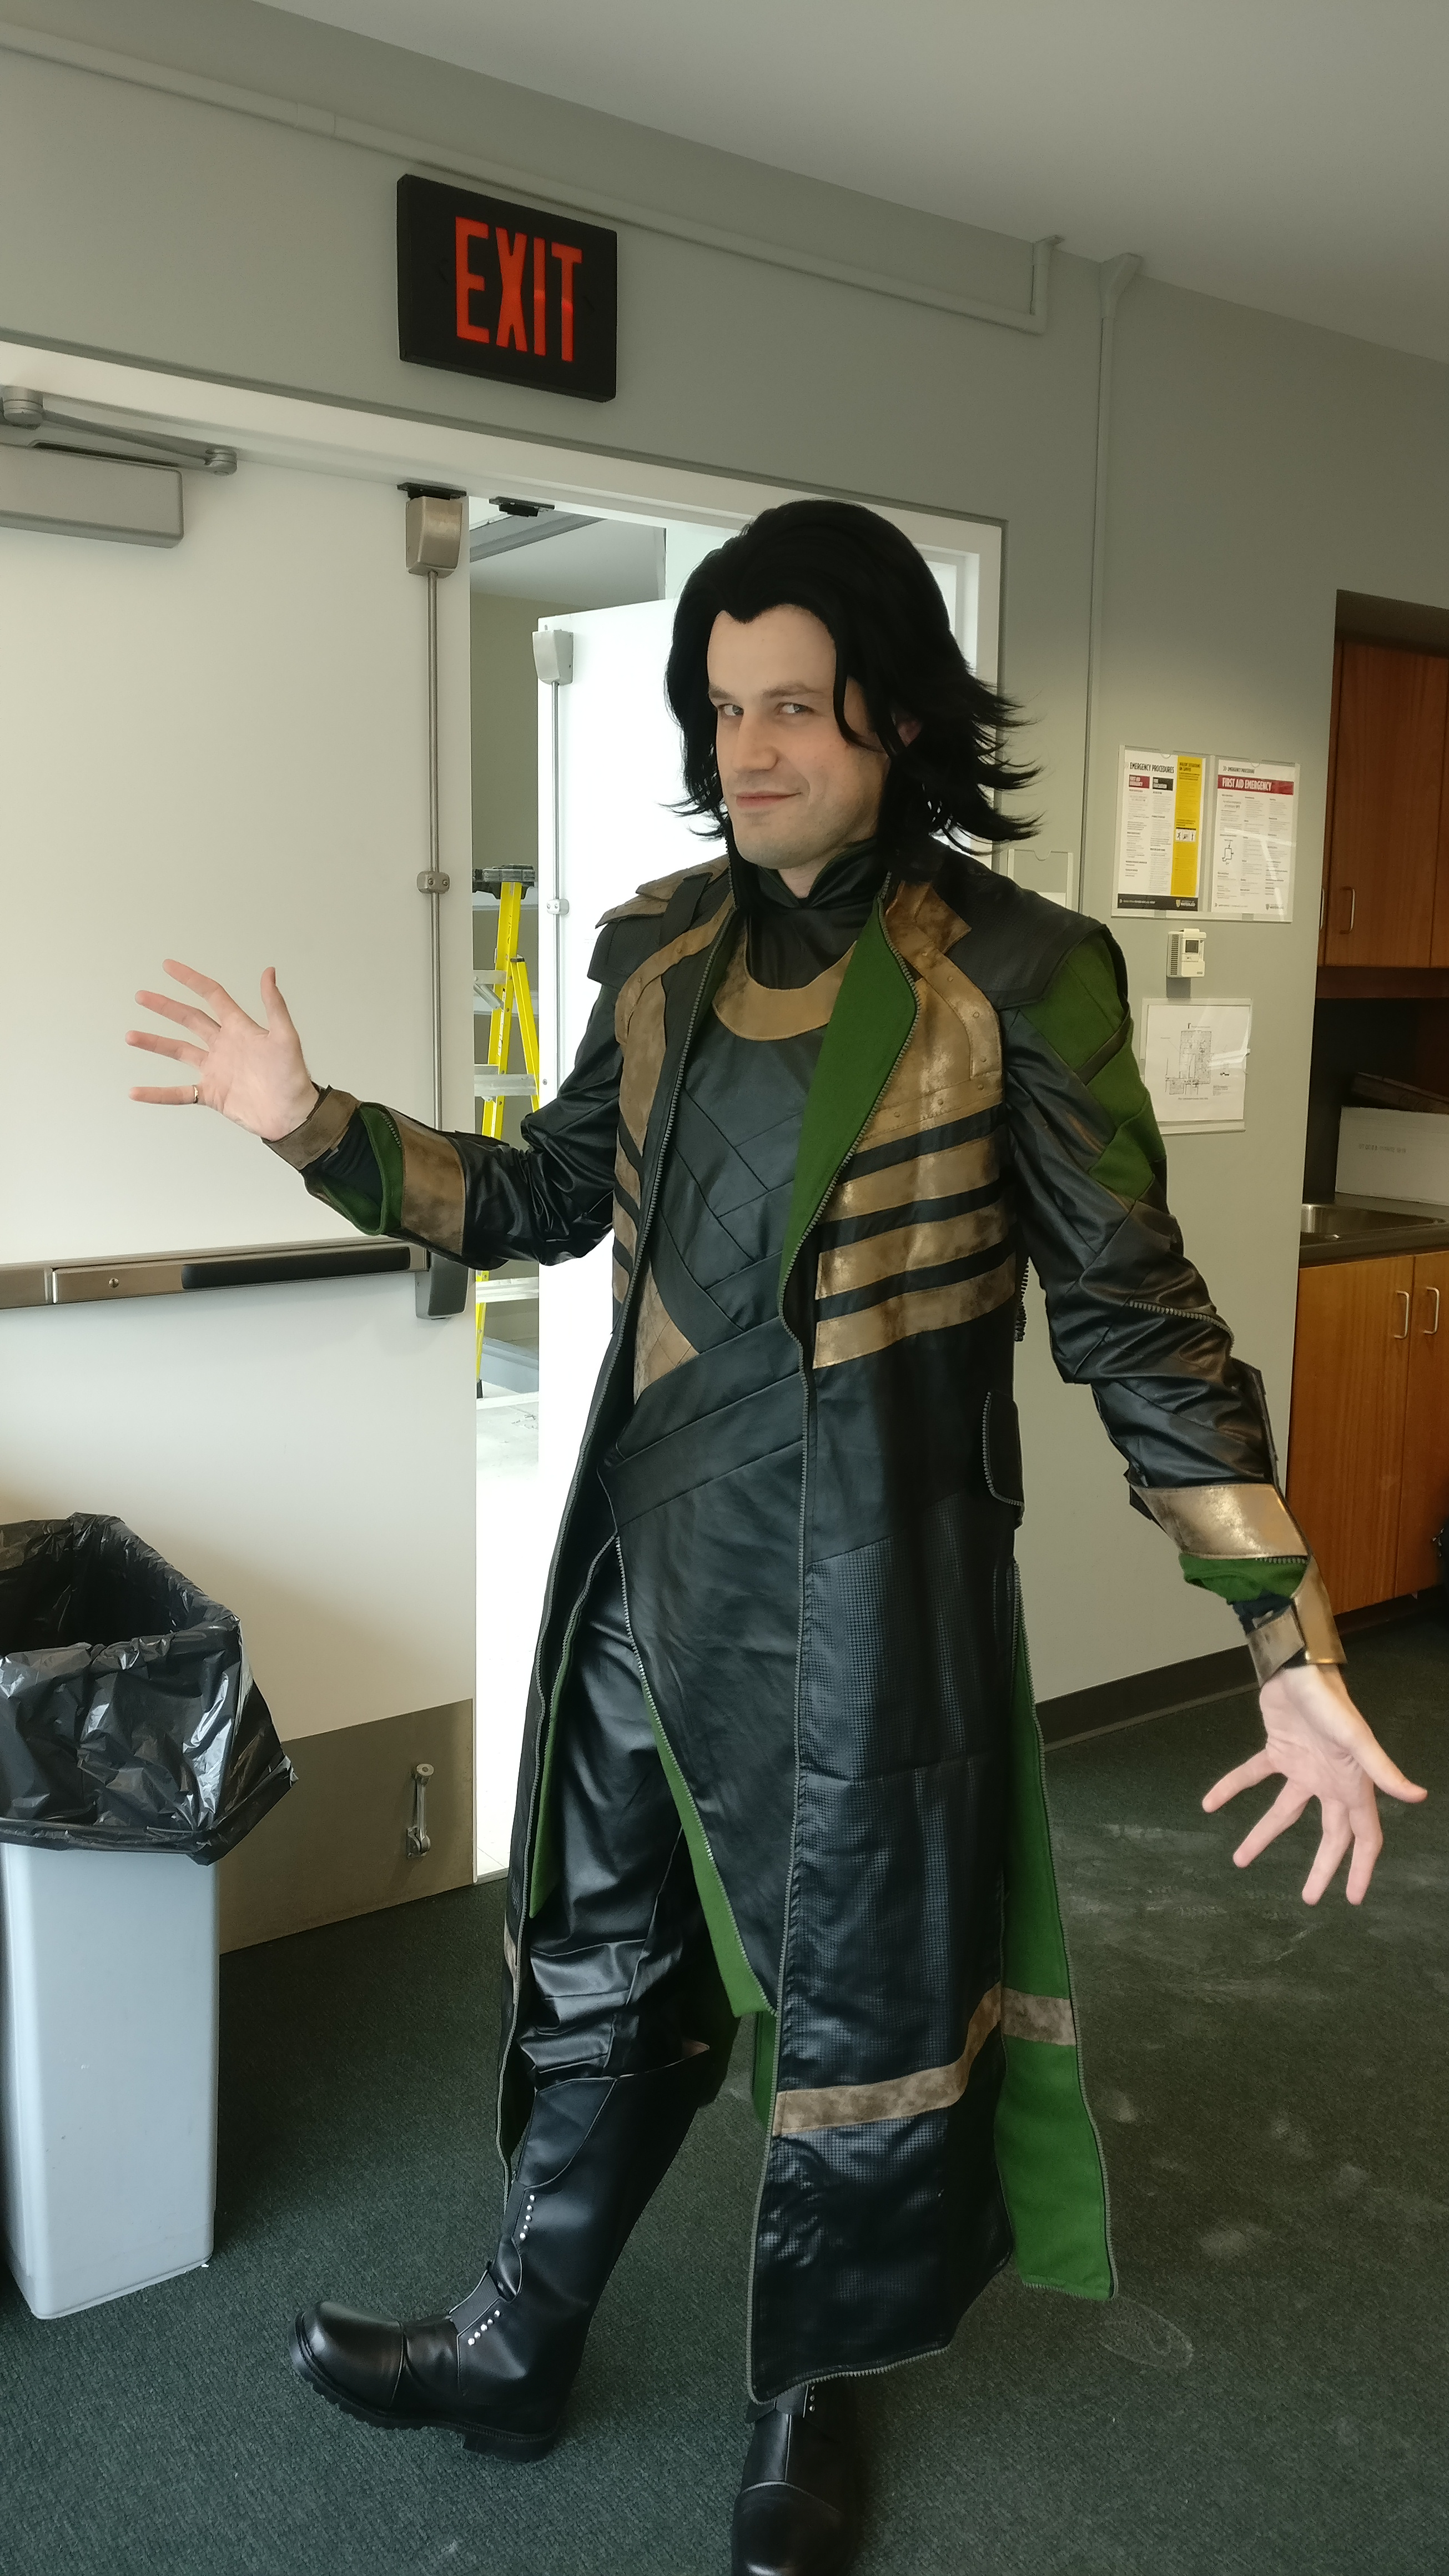
\includegraphics[width=0.4\textwidth]{images/Loki.jpg}
	\end{center}

\end{frame}


\begin{frame}
	\frametitle{Through the Bifrost}

	But all of these are analysis tools for your C and \Cpp programs.

	They are absolute murder on performance, but they are wonderful for finding errors in your program.

	To use them, start the tool of your choice and instruct it to invoke your program.

	The target program then runs under the ``supervision'' of the tool.

	Remember to enable debugging symbols in your compile.

\end{frame}

\begin{frame}
	\frametitle{Valgrind (memcheck)}

	Valgrind is the base name of the project and by default what it's going to do is run the memcheck tool.

	The purpose of memcheck is to look into all memory reads, writes, and to intercept and analyze every call to \texttt{malloc}/\texttt{free} and \texttt{new}/\texttt{delete}.

\end{frame}

\begin{frame}
	\frametitle{Is Your Program Worthy?}

	\begin{center}
		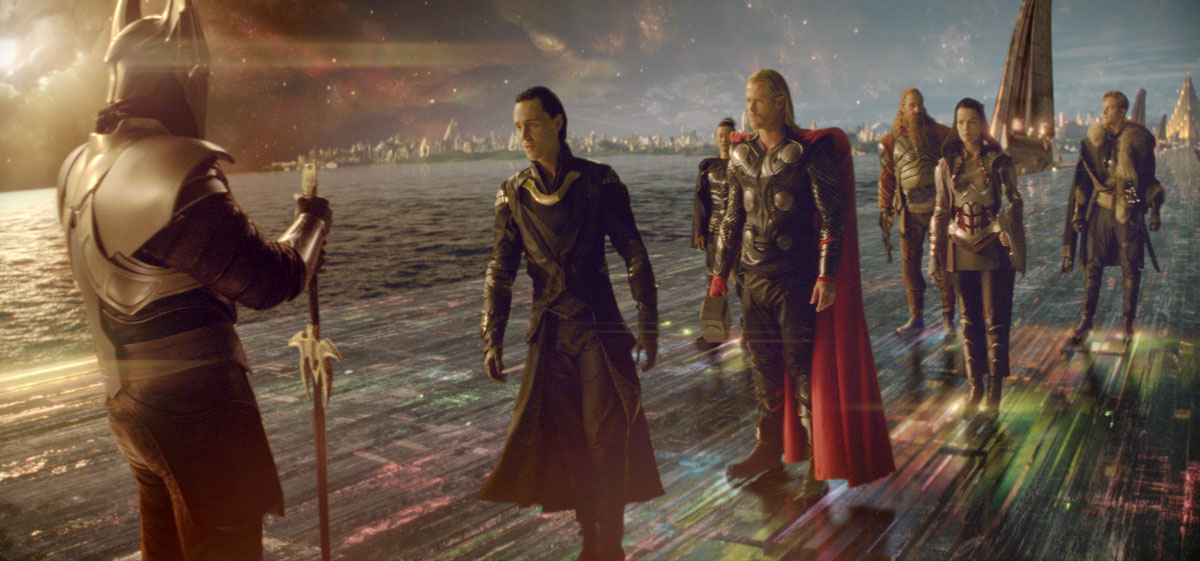
\includegraphics[width=\textwidth]{images/heimdall-waits.jpg}
	\end{center}

\end{frame}


\begin{frame}
	\frametitle{Is Your Program Worthy?}

	Memcheck can find problems like:
	\begin{itemize}
		\item Accessing uninitialized memory
		\item Reading off the end of an array
		\item Memory leaks
		\item Incorrect freeing of memory
		\item Incorrect use of C standard functions like \texttt{memcpy}
		\item Using memory after it's been freed.
		\item Asking for an invalid number of bytes in an allocation
	\end{itemize}

\end{frame}

\begin{frame}[fragile]
	\frametitle{Valgrind Output}
	{\scriptsize
		\begin{verbatim}
==8476== All heap blocks were freed -- no leaks are possible
\end{verbatim}
	}

That's the ideal. But is this realistic?
\end{frame}

\begin{frame}
	\frametitle{Send the Plumbers to the Watergate}


	Take the program's suggestion to use the \texttt{--leak-check=full}.

	You get a bit more detail about where you made the mistake.

	In the example below, lines 49 and 24 in the file \texttt{search.c} are the locations of the \texttt{malloc} calls that lack a matching call to \texttt{free}.

	It can't tell you where the call to \texttt{free} should go, only where the memory that isn't freed was allocated.

\end{frame}

\begin{frame}
	\frametitle{Reading the Output}

	\begin{itemize}
		\item \textbf{Definitely lost}
		\item \textbf{Indirectly lost}
		\item \textbf{Possibly lost}
		\item \textbf{Still reachable}
		\item \textbf{Suppressed}
	\end{itemize}

\end{frame}


\begin{frame}
\frametitle{Not My Problem?}

It's also important to learn what to ignore (or what's out of our hands). 

Example: it's thread creation or a library or similar. What do we do?

Consider carefully if we can do something about it!

Let's do some examples.

\end{frame}



\begin{frame}
	\frametitle{Helheim}

	\begin{center}
		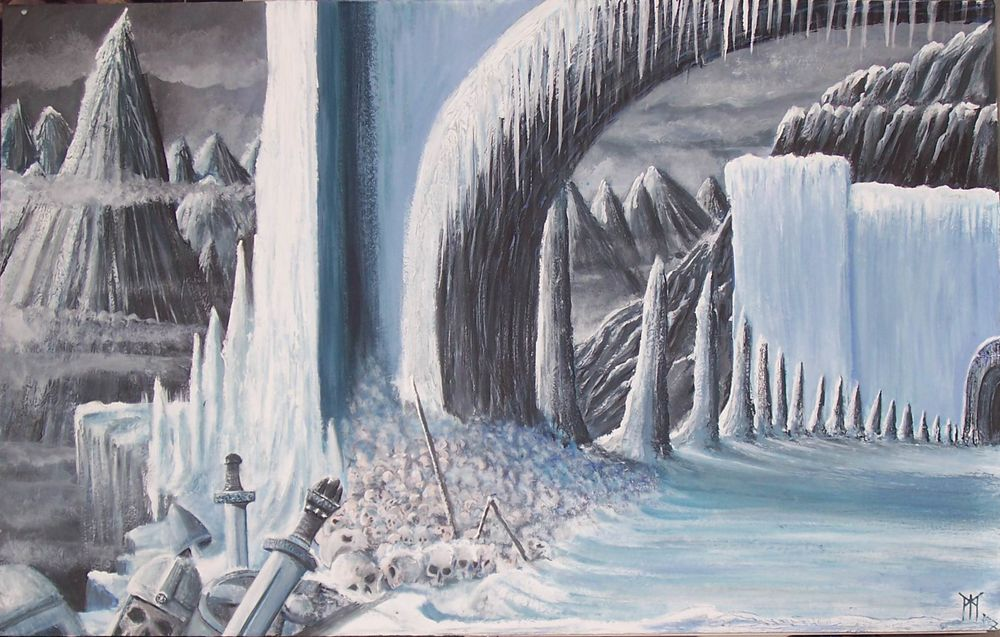
\includegraphics[width=\textwidth]{images/helheim.jpg}
	\end{center}

	\hfill Credit: Norse Legends Fandom User OlaTansta

\end{frame}


\begin{frame}
	\frametitle{What Fresh Hel is This}

	The purpose of Helgrind is to detect errors in the use of POSIX pthreads.

	In a way, Helgrind is a pretty neat tool for improving performance, even though it doesn't actually directly speed anything up.

	When we take single-threaded program and split it off into a multithreaded program, we may introduce a lot of errors.

	Humans are not very good at parallel thinking; we are very much sequential.

\end{frame}

\begin{frame}
	\frametitle{What Fresh Hel is This}

	But a program that is fast and wrong is probably less useful than one that is slow and correct.

	But can we make it faster and still have it be correct?

	That's the goal of Helgrind: determine where, if anywhere, there are concurrency problems.

	It can't prove that your program is correct (if only) but it can at least catch some of the common problems you might introduce when writing a parallel program.

\end{frame}

\begin{frame}
	\frametitle{Hel Hath No Fury...}

	Helgrind will categories errors into three basic categories:

	\begin{enumerate}
		\item Misuses of the pthreads API
		\item Lock ordering problems
		\item Data races
	\end{enumerate}


\end{frame}

\begin{frame}
	\frametitle{Misuse of the API}

	The first category does not require much explanation:


	\begin{itemize}
		\item Unlocking a mutex that is unlocked
		\item Deallocation of memory with a locked mutex in it
		\item Thread exit while holding a locked lock
	\end{itemize}
	... and many more.


\end{frame}

\begin{frame}[fragile]
	\frametitle{Type Two Errors}

	The second category of errors should be familiar to you:

	\begin{multicols}{2}
		\textbf{Thread P}
		\begin{verbatim}
	 1. wait( a ) 
	 2. wait( b )
	 3. [critical section]
	 4. signal( a )
	 5. signal( b )
  \end{verbatim}
		\columnbreak
		\textbf{Thread Q}
		\begin{verbatim}
	 1. wait( b ) 
	 2. wait( a )
	 3. [critical section]
	 4. signal( b )
	 5. signal( a )
  \end{verbatim}
	\end{multicols}
	\vspace{-2em}

	Potential Deadlock!

\end{frame}

\begin{frame}
	\frametitle{Interleaving Leaves Locks}

	Risk of deadlock:thread P holds mutex \texttt{a} and thread Q holds mutex \texttt{b}.

	Each waits for the mutex that the other one has.

	The example is slightly silly, of course, because it's super easy to see.

	There will not necessarily be an obvious (alphabetical) order.

\end{frame}

\begin{frame}
	\frametitle{Graph Theory Strikes Back}


	Helgrind builds a directed graph of lock acquisitions, so that when a thread acquires a lock, the graph is checked to see if a cycle exists.

	It will report as an error the initial order (the first order seen is the one viewed as ``correct'') and the the ``incorrect'' order that is the source of the potential problem.

	Really, though, all that matters is consistency.

\end{frame}


\begin{frame}
	\frametitle{Category 3}

	The third category we have discussed already.

	Recall the earlier definition of a race condition.

	Helgrind looks for when two threads access the same memory location without using locks.

\end{frame}

\begin{frame}
	\frametitle{Behind the Scenes}

	It examines the use of the standard threading primitives - lock, unlock, signal/post, wait...

	Anything that implies there might be an ordering between events is taken and added to a directed acyclic graph that represents these dependencies.

	If memory is accessed from two different threads and there is no path through this directed acyclic graph that indicates an ordering, then a race is reported.

	Although obviously at least one of these accesses must be a write.

\end{frame}

\begin{frame}[fragile]
	\frametitle{Name \& Shame}

	You can ask Helgrind to try to tell you about variable names (if it can) with the command line option \texttt{--read-var-info=yes}.

	\begin{verbatim}
==10454== Location 0x60104c is 0 bytes inside global var "var"
==10454== declared at datarace.c:3
\end{verbatim}

\end{frame}

\begin{frame}
	\frametitle{Fixing it Isn't My Problem}


	The authors of Helgrind assume that if it tells you where the problem is, you will figure out what variables are affected and how to properly prevent data races.

	\begin{center}
		
\includegraphics[width=0.3\textwidth]{images/its-your-job.jpg}
	\end{center}

	You might find this frustrating.

	Let's do some more examples.

\end{frame}

\end{document}

